\documentclass{article}
\usepackage[utf8]{inputenc}
\usepackage{scrextend}
\usepackage{graphicx}
\usepackage{float}


\title{Teoria Della Relatività Galileiana}
\author{Francesco Pio Cecca} 
\begin{document}
\maketitle
\section{Moti Relativi}

Con \textbf{moto relativo}, si intende un moto relativo ad un determinato sistema di riferimento. L'espressione chiave da usare è "rispetto a".\\\\
Il sistema di riferimento più ovvio che si possa considerare è un moto relativo rispetto alla Terra.\\
Noi tutti ci troviamo sulla Terra e, quando siamo seduti sul divano, diciamo di essere fermi. Nella nostra affermazione stiamo sottintendendo il fatto di essere fermi rispetto alla Terra e a tutto ciò che ci circonda: questo è il nostro sistema di riferimento abituale. D'altro canto, se siamo fermi rispetto alla Terra è ovvio che siamo in movimento rispetto al Sole e agli altri pianeti.\\\\
Ochhio però, dire che un corpo possiede un certo valore di velocità o si trova in una posizione particolare è un'informazione incompleta se non specifichiamo rispetto a cosa abbiamo misurato quella velocità o quella posizione.\\
\textbf{Tutti i moti sono moti relativi} rispetto a un fissato sistema di riferimento: dobbiamo cioè sempre specificare il sistema di riferimento usato per descrivere i fenomeni fisici che stiamo studiando.\\
Osservatori diversi in sistemi di riferimento diversi descrivono ciò che vedono in modo differente.\\\\
Anche la traiettoria di un corpo cambia nei moti relativi e a seconda del sistema di riferimento da cui si osserva il suo moto. Ad esempio, se una persona che viaggia in un vagone del treno lancia un pallina verso l'alto per poi riprenderla in mano, per lui la pallina avrà compiuto un semplice moto verticale in caduta libera, ma per un osservatore che si trova fermo sulla banchina la pallina avrà compiuto un moto parabolico perché la pallina, oltre che muoversi in verticale, si è spostata anche in orizzontale con la medesima velocità del treno.\\\\
\textbf{DOMANDA}: Le leggi della Fisica sono sempre le stesse in tutti i sistemi di riferimento oppure no?

\newpage
\section{Sistema Di Riferimento Inerziale}
Per definizione un sistema di riferimento \textbf{inerziale} è un sistema che si muove in moto rettilineo uniforme rispetto a un altro sistema, ossia con velocità costante rispetto ad esso.\\
Inoltre, in esso, è valida la seconda legge di Newton:
\begin{equation}
    \bar{F}=m\bar{a}
\end{equation}
Tale condizione viene a mancare quando la velocità non è più costante, ossia in presenza di una variazione di velocità.\\
Per definizione chiameremo sistema di riferimento \textbf{non inerziale} un sistema che accelera rispetto a un altro.
\section{Trasformazioni Di Galileo}
Dati due sistemi di riferimento inerziali, che si muovono dunque di moto rettilineo uniforme l'uno rispetto all'altro, quali sono le formule che ci permettono di calcolare la posizione di un corpo in uno dei due sistemi conoscendo la posizione nell'altro?\\\\
Partiamo da un semplice esempio per il caso unidimensionale. Siamo fermi sulla banchina di una stazione ferroviaria e, al passaggio di un treno che procede a \underline{velocità costante}, notiamo su di esso un nostro amico (Marco).
\begin{figure}[H]
    \centering
    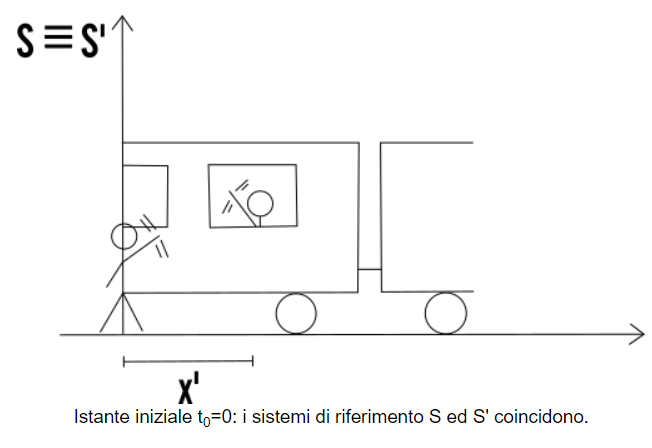
\includegraphics[scale=0.5]{Trasformazioni di galileo 1.png}
    \label{fig:my_label}
\end{figure}
\noindent
Consideriamo come istante iniziale $t_{0}=0$ l'istante di tempo in cui incrociamo lo sguardo con Marco. Consideriamo inoltre la stazione come il nostro sistema di riferimento (S) e il treno, su cui si trova Marco, come secondo sistema di riferimento (S').\\
Poiché il treno viaggia in in moto rettilineo uniforme rispetto alla stazione, sappiamo per definizione che S ed S' sono sistemi di riferimento inerziali.\\
Per come abbiamo scelto i sistemi di riferimento, nell'istante iniziale $t_{0}=0$ le origini di entrambi i sistemi coincidono e Marco si trova ad un distanza da noi pari a x', che è anche la distanza di Marco rispetto all'origine del suo sistema di riferimento.\\
Col passare dei secondi Marco si allontana assieme al treno con una velocità costante pari a v.\\
\begin{figure}[H]
    \centering
    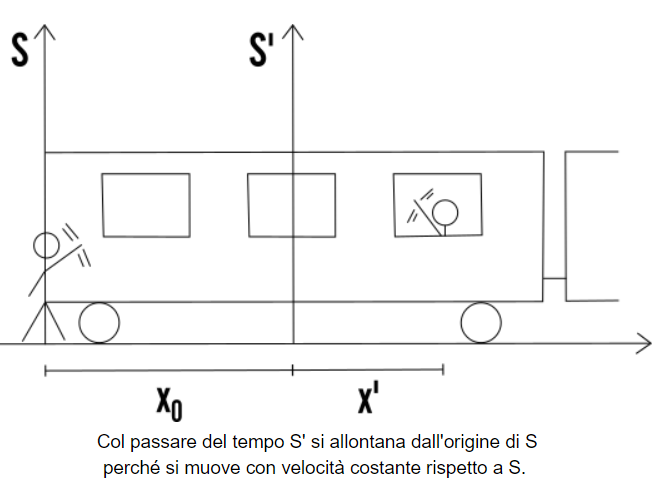
\includegraphics[scale=0.4]{Trasformazioni di galileo 2.png}
    \label{fig:my_label}
\end{figure}
\noindent
Abbiamo tutto quello che ci serve per ricavare la formula di trasformazione galileiana, ossia la legge per calcolare la posizione x' nel sistema di riferimento S' a partire dalla posizione x nel sistema di riferimento S.\\
In accordo con le formule per il moto rettilineo uniforme, dopo un tempo t l'origine del sistema di riferimento S' del treno si sarà spostata di una lunghezza data da:
\begin{equation}
    x_{0}=vt
\end{equation}
rispetto all'origine del sistema S..\\
 Rispetto a noi, che ci troviamo sulla banchina, Marco al tempo t si trova a una distanza che è la somma::
 \begin{itemize}
     \item della sua posizione rispetto all'origine di S', ossia x'
     \item della distanza percorsa dall'origine di S' rispetto all'origine di S al tempo t.
 \end{itemize}
In una formula:
\begin{equation}
    x=x'+x_{0} \,\,\,\,\,\,\,\,\,\,\,\,\,\, x'=x-vt
\end{equation}
Volendo esprimere le trasformazioni di Galileo in due o tre dimensioni, otterrei:
\begin{figure}[H]
    \centering
    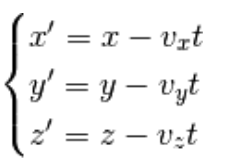
\includegraphics[scale=0.4]{Trasformazioni di galileo 3.png}
    \label{fig:my_label}
\end{figure}
\noindent
Se considerassimo due sistemi non inerziali, ossia tali per cui l'uno accelera rispetto all'altro, il ragionamento precedente cesserebbe di valere.\\
Non potremmo infatti usare le formule per il moto rettilineo uniforme per calcolare lo spostamento dell'origine del sistema S' rispetto all'origine del sistema S.
\newpage
\section{Composizione Della Velocità}
Quando siete di fretta e dovete prendere la metro, cosa fate? Con ogni probabilità scendete di corsa lungo le scale mobili, in modo da sommare alla velocità delle scale la velocità della vostra corsa. In questo modo riuscite ad arrivare in fondo prima.\\
Per un osservatore esterno, situato sulla banchina e fermo rispetto alla scala mobile, la velocità con cui vi state muovendo è data dalla somma della velocità costante delle scale mobili e della velocità della vostra corsa. Nel sistema delle scale mobili invece vi state muovendo semplicemente con la vostra velocità, e le persone che si lasciano trasportare giù appoggiate al corrimano sono ferme.\\
Quindi, anche la velocità è relativa e dipende dal sistema di riferimento. Si parla così di \textbf{velocità relativa} rispetto al sistema di riferimento considerato.\\\\
Esiste una relazione matematica che ci permette di calcolare la velocità v rilevata da un osservatore in un sistema di riferimento S, a patto di conoscere la velocità v' rilevata da un osservatore in un sistema S' inerziale rispetto al primo.\\\\
Tale formula prende il nome di formula di composizione delle velocità e ribadiamo che è valida solamente se si considerano sistemi di riferimento inerziali. Per semplicità consideriamo dapprima il caso di due sistemi monodimensionali e, dopo aver fissato un verso per le ascisse crescenti, possiamo scrivere la relazione:
\begin{equation}
    \bar{v}=\bar{v_{0}+\bar{v'}}
\end{equation}
dove:
\begin{itemize}
    \item $\bar_{v}$ è la velocità rilevata dall'osservatore situato nel sistema S
    \item $\bar{v'}$ viene detta velocità relativa, ed è la velocità rilevata dall'osservatore situato nel sistema S'
    \item $\bar{v_{0}}$ viene detta velocità di trascinamento ed è la velocità (costante per ipotesi) di S' rispetto a S
\end{itemize}
Se esplicitiamo la velocità rilevata nel sistema S' otteniamo la legge di composizione inversa delle velocità, detta \textbf{formula per la velocità relativa}:
\begin{equation}
    \bar{v'}=\bar{v}-\bar{v_{0}}
\end{equation}
Le leggi che abbiamo appena scritto sono vettoriali e valgono in una, due e tre dimensioni. Esattamente come nel caso della posizione, possiamo scrivere le equazioni componente per componente nel caso tridimensionale:
\begin{figure}[H]
    \centering
    \includegraphics[scale=0.5]{Composizione Velocità 1.png}
    \label{fig:my_label}
\end{figure}
\newpage
\section{Principio Di Relatività Galileiana}
Sappiamo che sia la posizione sia la velocità dipendono dal sistema di riferimento scelto.\\
Dalle leggi di trasformazione galileiane e dalle formule di composizione delle velocità sappiamo inoltre come calcolare la posizione e la velocità nel passaggio da un sistema di riferimento inerziale ad un altro.\\
DOMANDA: anche l'accelerazione cambia? No, \textbf{in qualunque sistema inerziale l'accelerazione è sempre la stessa}.
\begin{equation}
    \frac{d\bar{v'}}{dt}=\frac{d\bar{v}}{dt}\,\,\,\,\,\,\,\,\,\,\,\ a=a'
\end{equation}
Inoltre, la seconda legge di Newton ci dice che la forza è data dal prodotto della massa per l'accelerazione. Se in due sistemi di riferimento inerziali le accelerazioni sono uguali, significa che anche le forze misurate in questi due sistemi sono uguali.
\begin{equation}
    F=F'
\end{equation}
Ecco allora che siamo giunti a quello che viene più comunemente enunciato come \textbf{principio di relatività di Galileo}: in tutti i sistemi di riferimento inerziali le leggi della dinamica newtoniana restano invariate.\\
QUINDI: l'invarianza dell'accelerazione si traduce nell'invarianza delle leggi della Dinamica, a patto che in entrambi i casi si considerino sistemi di riferimento inerziali.

 
\end{document}
